\section*{Exercice 189 -- Modélisation}
\setcounter{exo}{0}
%CCS PSI 2005


\begin{obj}
Vérifier les performances de l’asservissement d’inclinaison par rapport à la verticale.
\end{obj}

Pour une utilisation confortable et sûre, le Segway doit satisfaire les performances
énoncées dans le tableau extrait du cahier des charges.
\begin{center}
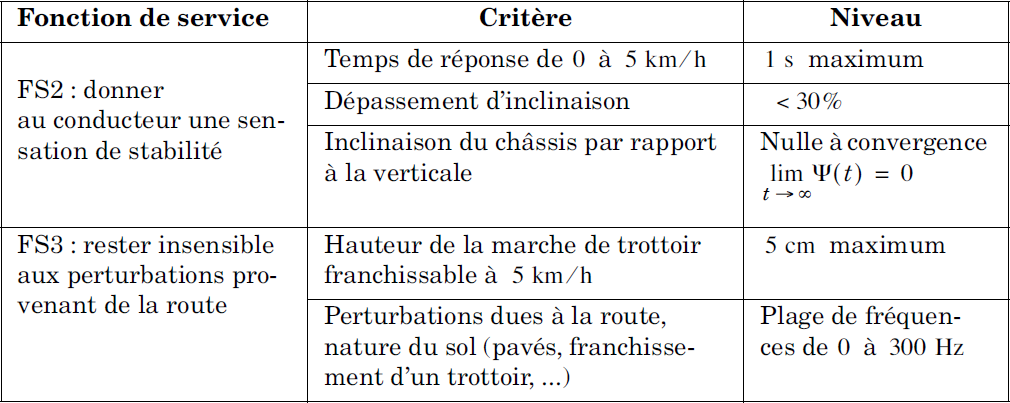
\includegraphics[width=\linewidth]{976_01}%
\end{center}
La régulation d’inclinaison du Segway® est réalisée par :
\begin{itemize}
\item un moto-réducteur qui permet de délivrer un couple $C_m(t)=K_m u(t)$ où $u(t)$ est une grandeur de commande et $K_m=\SI{24}{N.m.V^{-1}}$;
\item le système mécanique dont les équations, dans le cas où l’angle $\alpha(t)$ n’est pas supposé constant, se met
sous la forme :
$\left\{
\begin{array}{l}
\dot{V}(t)=\dfrac{1}{D}\left( B\ddot{\chi}(t)+2\dfrac{C_m(t)}{R}\right) \\
\left(DA-B^2\right)\ddot{\chi}(t)=2\left(\dfrac{B}{R}+D\right)C_m(t)+DC\chi(t)
\end{array}
\right.
$ 
avec
$\left\{
\begin{array}{l}
A=\SI{90}{kg.m^2} \\
B=\SI{75}{kg.m} \\
C=\SI{750}{kg.m^2.s^{-2}} \\
D=\SI{125}{kg} \\
R=\SI{240}{mm} \\
\chi(t)=\alpha(t)+\psi(t) 
\end{array}
\right.
$ 
\end{itemize}

\subparagraph{}
\textit{}
\ifprof
\begin{corrige}
\end{corrige}
\else
\fi



\begin{enumerate}
\item ...
\end{enumerate}